\documentclass[11pt]{article}
\usepackage[margin=1in]{geometry}
\usepackage{graphicx}
\usepackage{amsmath}
\usepackage{booktabs}
\usepackage{xcolor}
\usepackage{listings}
\usepackage[colorlinks=true,linkcolor=blue,urlcolor=blue]{hyperref}
\usepackage{caption}
\captionsetup{font=small}

\lstset{basicstyle=\ttfamily\small,breaklines=true,columns=fullflexible,frame=single,
        backgroundcolor=\color{gray!8}}

\title{\textbf{PERSONA--CPG--MuJoCo}\\[2pt]
\large Personalizing a biologically detailed spiking CPG to a rat hindlimb}
\author{KinematicsCPG}
\date{\today}

\begin{document}
\maketitle

\tableofcontents

\section{Overview}
\label{sec:overview}

This project personalizes a biologically detailed spiking central pattern
generator (CPG) so that a simulated rat hindlimb reproduces reference
locomotion kinematics. The CPG is a NEST network; the limb is a MuJoCo model;
the optimization is \emph{PERSONA}
(\textbf{P}arameter \textbf{E}xploration and \textbf{R}einforcement via
\textbf{N}atural-gradient approximation): an online natural-gradient /
Fisher-matrix search over the CPG's neuronal, synaptic and connectivity
parameters.

The personalization objective is for the \emph{controlled} hindlimb's ankle
angle to track a mocap-driven \emph{target} hindlimb through a locomotion
bout. Biological plausibility is checked against a published rat
split-belt-treadmill dataset.

\section{Repository layout}
\label{sec:layout}

\begin{table}[h]
\centering
\begin{tabular}{ll}
\toprule
Path & Responsibility \\
\midrule
\texttt{persona/} & PERSONA framework: parameters, registry, Fisher/strategy, agent, orchestrator, validation \\
\texttt{t2xcpg/} & The two-leg spiking CPG (NEST), registered through the PERSONA \texttt{Registry} \\
\texttt{model/} & MuJoCo biomechanics: bilateral rig adapter, afferent models (CUT/Ia/Ib) \\
\texttt{loader/} & Zenodo mocap loader (marker$\rightarrow$angle) and locomotion statistics \\
\texttt{personalize.py} & Entry point: builds and runs the closed loop, writes logs and figures \\
\texttt{dual\_rat\_hindlimb.xml} & Bilateral MuJoCo model (controlled L/R + target L/R) \\
\texttt{docs/} & Design spec, plan, this document, figures \\
\texttt{tests/} & pytest suite \\
\texttt{tinycpg/, memcpg/} & Reference implementations only (not modified) \\
\bottomrule
\end{tabular}
\caption{Repository layout.}
\end{table}

\section{Installation}
\label{sec:install}

The runtime is a Python~3.12 virtual environment under WSL (Ubuntu) with:
NEST~3.10, MuJoCo~3.14, NumPy~2.5, SciPy~1.18, pandas~3.0, h5py~3.16,
matplotlib~3.11, pytest.

\begin{lstlisting}
# from the repository root, inside the WSL venv
python -c "import nest, mujoco; print(nest.__version__, mujoco.__version__)"
python -m pip install pytest
\end{lstlisting}

\section{Usage}
\label{sec:usage}

Run the full two-stage personalization (builds the network, runs the loop,
writes \texttt{run\_log.csv}, \texttt{run\_log.npz}, \texttt{validation\_results.png}):

\begin{lstlisting}
python personalize.py
\end{lstlisting}

Programmatically:

\begin{lstlisting}
from personalize import run_personalization, DEFAULT_REFERENCE, DEFAULT_STATS
res = run_personalization(reference_path=DEFAULT_REFERENCE,
                          stats_path=DEFAULT_STATS,
                          output_dir="out", n_steps=200, verbose=True)
print(res["acceptable"], res["angle_coverage"])
\end{lstlisting}

Run the tests:

\begin{lstlisting}
python -m pytest
\end{lstlisting}

\paragraph{Outputs.} \texttt{run\_log.csv} (per-step table: time, model/target
ankles, loss, advantage, muscle drives, afferent rates, phase, stage),
\texttt{run\_log.npz} (same as arrays), \texttt{validation\_results.png}
(tracking + learning), and \texttt{tracking.png}, \texttt{learning.png}.

\section{Pipeline}
\label{sec:pipeline}

Each control step performs the following (Figure~\ref{fig:arch}):

\begin{enumerate}
  \item \textbf{Sample} an exploratory mean for every registered parameter from
        its controlling standard deviation $\sigma_{\text{ctrl}}$.
  \item \textbf{Apply} the sampled parameters to the live NEST network through
        the \texttt{Registry} (weights, probabilities, rates, Izhikevich
        parameters), and re-sample per-neuron biological dispersion from
        $\sigma_{\text{param}}$.
  \item \textbf{Simulate} the CPG for $dt$ and step the MuJoCo rig; read muscle
        drives out and sensory afferents back.
  \item \textbf{Score}: vector error between model and target ankle angles,
        per-leg phase (stance/swing) moving-average baselines, component-wise
        advantage.
  \item \textbf{Update}: natural-gradient step
        $\Delta\mu=\eta\,F^{-1}\,\text{score}\cdot\text{advantage}$, with $F$ the
        empirical correlation matrix over parameters \emph{and} noise features
        (Poisson-rate deltas and STDP weight deltas).
\end{enumerate}

\begin{figure}[h]
\centering
\fbox{\parbox{0.92\textwidth}{\centering
\texttt{MocapLoader} $\rightarrow$ \texttt{MocapTargetDriver} (target ankle/hip/knee)
$\rightarrow$ \texttt{Rig.step} \\
$\uparrow$ \hspace{2.6in} $\downarrow$ \\
\texttt{Agent.sample\_actions()} $\rightarrow$ \texttt{Registry.apply} $\rightarrow$
\texttt{L2CPG.update/step} $\rightarrow$ \texttt{Registry} $\rightarrow$
\texttt{Agent.step(loss)}}}
\caption{Closed-loop data flow implemented in \texttt{personalize.py}.}
\label{fig:arch}
\end{figure}

\subsection{Two-stage protocol}
\textbf{Stage 1 (``pose'')} holds the target at the trial's initial pose until
the model's two ankle errors stay below \texttt{eps\_pose} for
\texttt{pose\_hold\_steps}. \textbf{Stage 2 (``track'')} follows the mocap
trajectory and stops early when the windowed-mean loss drops below
\texttt{loss\_stop}.

\section{Models}
\label{sec:models}

\paragraph{PERSONA (\texttt{persona/}).}
\texttt{PersonaParam} carries a mean and two standard deviations:
$\sigma_{\text{ctrl}}$ (exploration/exploitation, also updated by a
policy-gradient variance rule) and $\sigma_{\text{param}}$ (biological
dispersion across neurons). \texttt{FisherMatrix} builds a unit-diagonal
correlation matrix by proportional shrinkage $(1-\lambda)C+\lambda I$ over a
rolling window of standardized feature perturbations, and maps the
natural-gradient step back to physical units via the recorded per-feature
scales. Noise features (Poisson-rate and STDP-weight deltas) enter through
$F^{-1}$.

\paragraph{CPG (\texttt{t2xcpg/}).}
A two-leg network per the circuit scheme: rhythm generators RGE/RGF with
reciprocal inhibition through InE/InF; motor pools M-E/M-F; Renshaw cells
R-E/R-F; separate \textbf{Ia} (length/velocity, stretch reflex) and
\textbf{Ib} (force/activation, autogenic inhibition) afferents; cutaneous
\textbf{CUT} (stance reinforcement); commissural V2a/V0v/V0d/V3-F/In1; a
brainstem drive BS$\rightarrow$RGE/RGF. All populations and connections are
created through the PERSONA \texttt{Registry}; STDP is used on the sensory
input pathways (CUT$\rightarrow$RGE, Ia$\rightarrow$RG). No afferent is
timer-driven.

\paragraph{Biomechanics (\texttt{model/}).}
A bilateral MuJoCo rig with four limbs: controlled~L/R (SOL/TA muscles plus
position servos on every non-ankle joint) and mocap-driven target~L/R. Only
the ankle is muscle-driven (MVP); \texttt{CPGInput}/\texttt{CPGOutput} carry
the full bilateral sensory/motor state.

\paragraph{Data (\texttt{loader/}).}
Zenodo split-belt-treadmill mocap (markers IC, GT, KN, EA, MH per side) is
converted to sagittal joint angles by planar marker triples, aligned to the
sim rest pose, and cropped/resampled to the simulation $dt$. The statistical
table supplies global locomotion parameters (duty factor, double support,
step/stride length, synergy contributions) for validation.

\section{Current run}
\label{sec:run}

A 200-step run on the RatA tied trial produced the following (new per-step
logging enabled). The optimizer does \emph{not} yet reduce the loss; the
figures below show why.

\begin{table}[h]
\centering
\begin{tabular}{ll}
\toprule
Quantity & Value \\
\midrule
Stage reached & \texttt{pose} only (0 track steps) \\
Drive saturation (E / F) & $0.995$ / $0.995$ of steps at $1.0$ \\
Target ankle (L) & constant $+1.148$ rad \\
Model ankle (L) range & $0.000$ to $+0.480$ rad \\
CUT afferent (max) & $0$ Hz (no paw contact) \\
Ib afferent (max) & $192$ Hz (at ceiling) \\
Loss (first-20 / last-20 mean) & $0.899$ / $0.853$ (no trend) \\
\bottomrule
\end{tabular}
\caption{Outcome of the current 200-step run.}
\end{table}

\begin{figure}[h]\centering
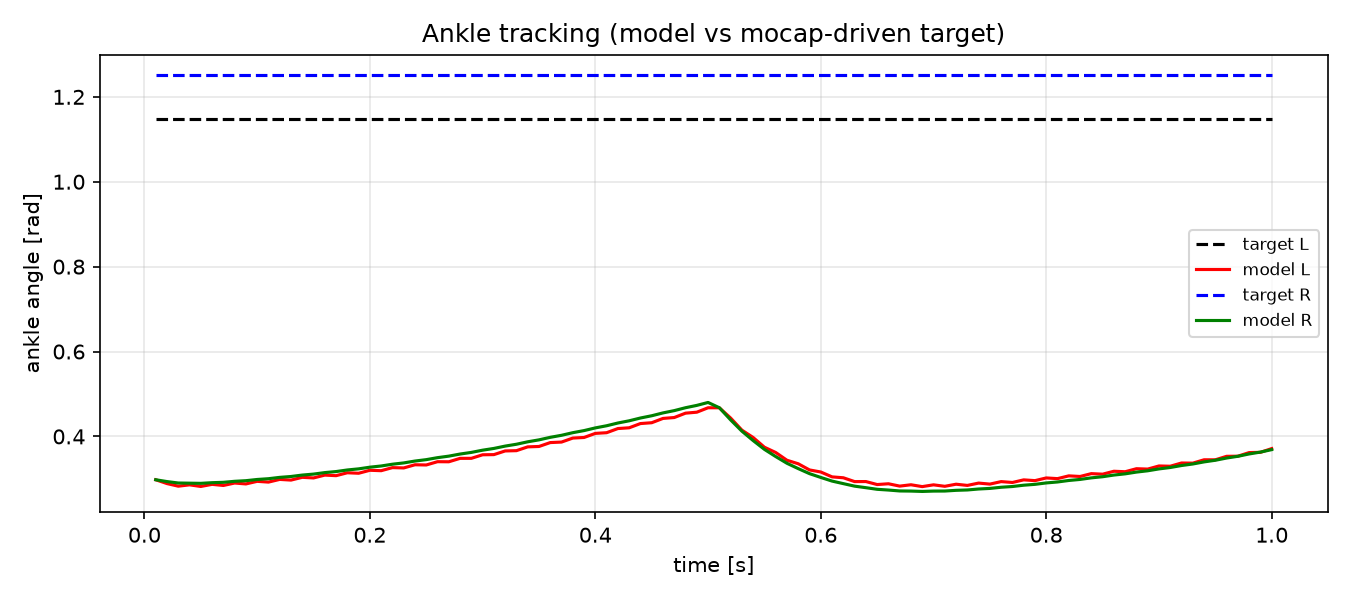
\includegraphics[width=0.85\textwidth]{figures/fig_tracking.png}
\caption{Ankle tracking: the target is a constant unreachable value; the model
ankle oscillates around rest.}
\end{figure}

\begin{figure}[h]\centering
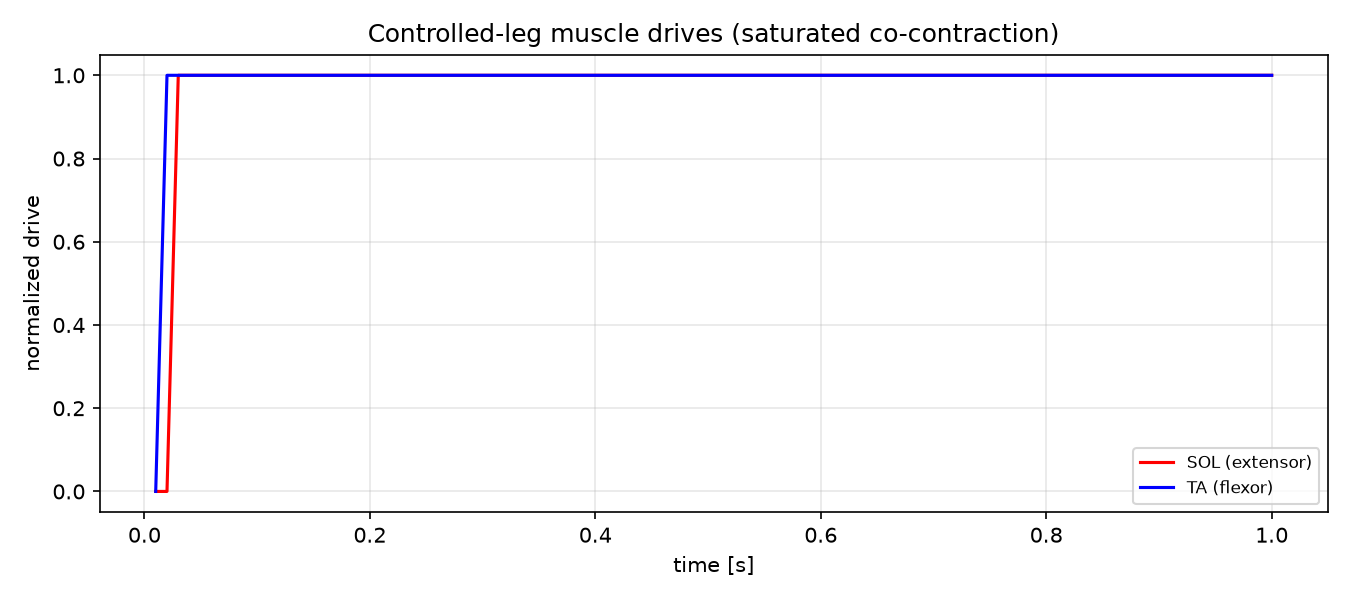
\includegraphics[width=0.85\textwidth]{figures/fig_drives.png}
\caption{Controlled-leg muscle drives: SOL and TA pinned near $1.0$
(co-contraction).}
\end{figure}

\begin{figure}[h]\centering
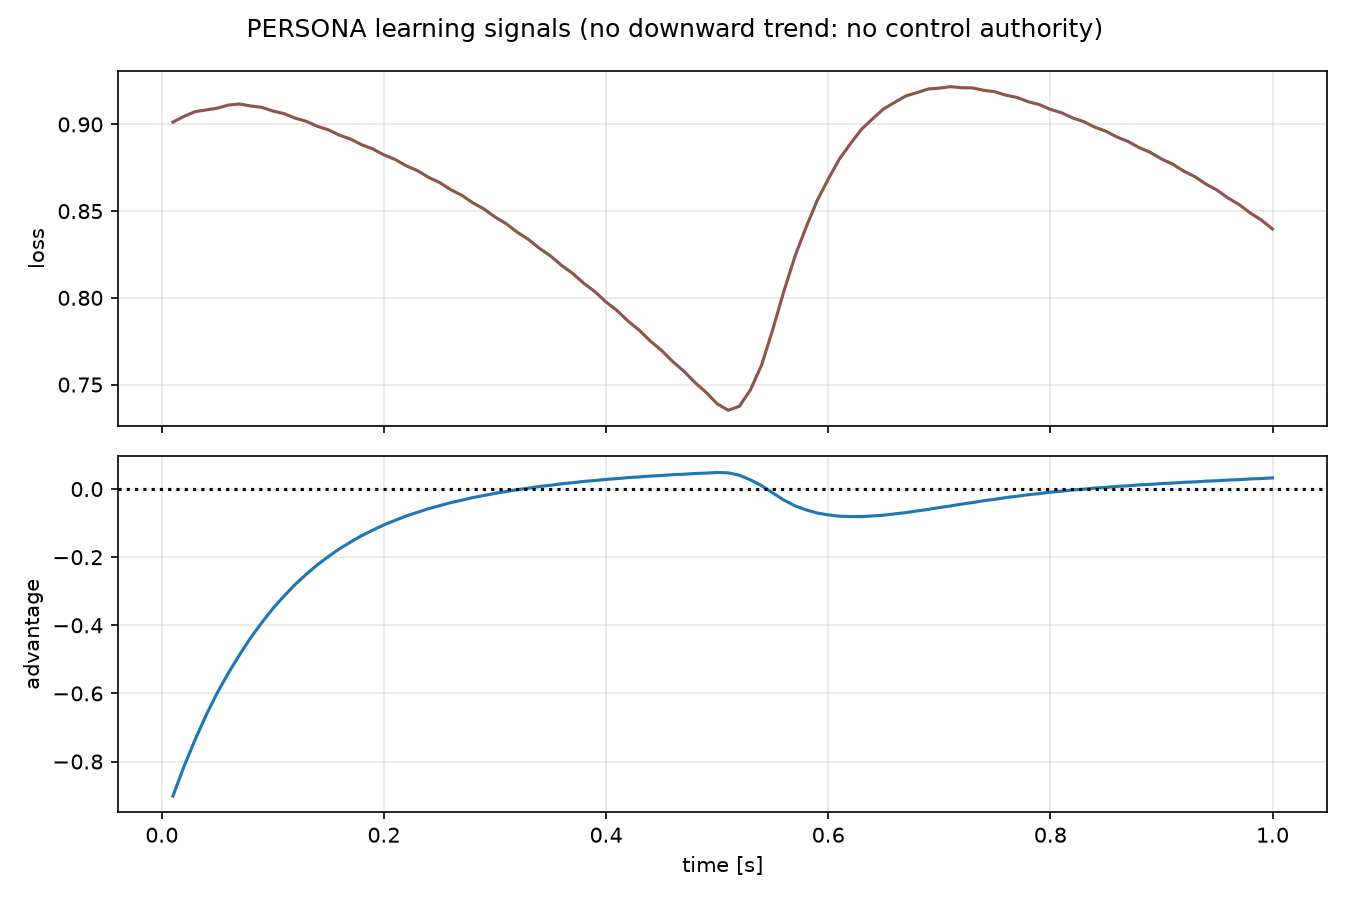
\includegraphics[width=0.85\textwidth]{figures/fig_learning.png}
\caption{Loss and advantage: no sustained downward trend.}
\end{figure}

\begin{figure}[h]\centering
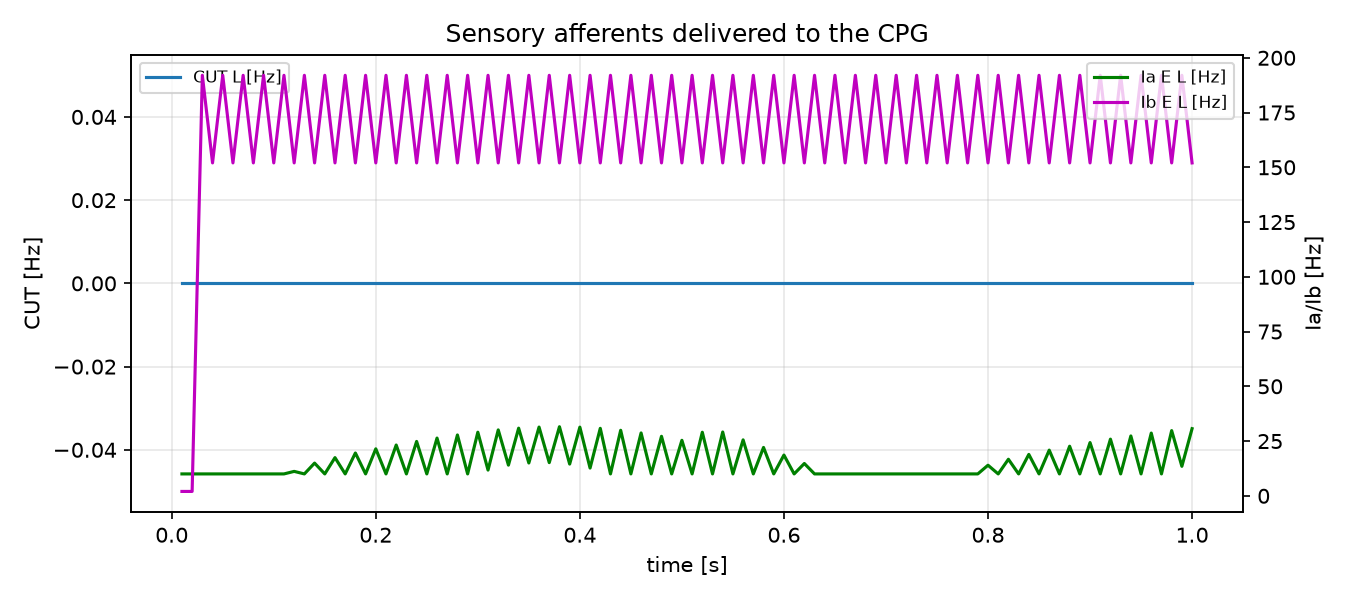
\includegraphics[width=0.85\textwidth]{figures/fig_afferents.png}
\caption{Afferents: CUT flat at $0$; Ib pinned at its ceiling.}
\end{figure}

\section{Status and known issues}
\label{sec:status}

The implementation is complete and unit-tested and executes end to end, but it
does not yet personalize because the plant gives the optimizer no authority.
Three defects compound:

\begin{enumerate}
  \item \textbf{Muscle readout saturates.} The drive threshold
        $\text{max\_spikes}=n_{\text{mn}}\cdot dt/5 = 20$ is far below the motor
        pools' $90$--$260$ spikes per $10$~ms, so both drives clip to $1.0$
        ($\sim\!99.5\%$ of steps), the limb co-contracts, and parameter changes
        barely move the ankle.
  \item \textbf{Target is a constant, unreachable pose.} \texttt{align\_to\_sim}
        followed by \texttt{fit\_to\_joint\_range} moves the initial pose to
        $+1.148$; Stage~1 never converges and Stage~2 never starts.
  \item \textbf{Sensory loop is dead.} The paw rests above the treadmill plane
        (no contact $\Rightarrow$ CUT$=0$), while co-contraction saturates Ib.
\end{enumerate}

\section{Further improvements}
\label{sec:future}

\subsection*{P0 --- restore control authority (blocking)}
\begin{enumerate}
  \item Recalibrate the drive readout from a measured per-neuron reference rate
        (or normalize each pool by its running max) so drives span $[0,1]$ with
        a broad histogram rather than clipping.
  \item Give the muscles authority: increase \texttt{force}/\texttt{scale}, or
        start from a standing offset so the ankle can reach the target band.
  \item Make the target moving and reachable: center (offset) the aligned
        trajectory instead of stretching it into the joint limit, and ensure
        Stage~1 converges; verify Stage~2 is entered.
\end{enumerate}

\subsection*{P1 --- repair the sensory loop}
\begin{enumerate}
  \item Establish ground contact (pelvis height / initial pose / reference
        limb); verify CUT$>0$ during stance.
  \item Cap Ib / lower \texttt{k\_force} so Ib varies; re-check the
        autogenic-inhibition sign.
  \item Add a leaky integrator to the readout for smooth, time-differentiable
        drives.
\end{enumerate}

\subsection*{P2 --- make PERSONA personalize}
\begin{enumerate}
  \item Add physics regression tests that \emph{fail} on the current behavior:
        drives not saturated, CUT$>0$ in stance, Stage~2 entered, and
        $\text{loss}_{last}<\text{loss}_{first}$ on a sinusoidal target.
  \item Probe control authority ($\partial\text{ankle}/\partial\text{param}$)
        before trusting the optimizer; prune the optimization subspace (274
        features with a short window makes $F$ rank-deficient and the step
        essentially ridge-SGD).
  \item Reduce per-step cost ($\sim\!6.5$~s/step) and stage the study:
        (a) drive actuators directly, (b) fixed CPG params showing anti-phase
        SOL/TA, (c) then PERSONA on top.
\end{enumerate}

\subsection*{P3 --- validation and reporting}
\begin{enumerate}
  \item Log per-neuron rates and $F$ condition number per step.
  \item Add a gait-quality gate (minimum stance/swing cycles) before the
        acceptance rule.
  \item Replace the ankle-angle step/stride proxies with foot-position
        excursions in mm to match the statistics table.
\end{enumerate}

\section{References}
\label{sec:refs}

\begin{itemize}
  \item Fujiki et al. \emph{Dataset of measured kinematics \ldots\ rat hindlimb
        locomotion during split-belt treadmill walking}, Zenodo, 2025.
        DOI: 10.5281/zenodo.17310509.
  \item Danner et al. \emph{Spinal control of locomotion before and after
        spinal cord injury}, Exp.\ Neurol., 2023. DOI: 10.1016/j.expneurol.2023.114496.
\end{itemize}

\end{document}